\documentclass[12pt,letterpaper]{article}

\usepackage{amsmath, amsthm, amsfonts, amssymb}
\usepackage{graphicx,hyperref}
\usepackage{microtype, parskip}
\usepackage[numbers,sort&compress]{natbib}
\usepackage{lineno}
\usepackage{docmute}
\usepackage[font=small]{caption}
\usepackage{subcaption, multirow, morefloats}
\usepackage{wrapfig, rotating}
\usepackage{titlesec}
\usepackage{authblk, attrib, fullpage}
\usepackage{lineno}

\frenchspacing

\captionsetup[subfigure]{position = top, labelfont = bf, textfont = normalfont, singlelinecheck = off, justification = raggedright}

\begin{document}
\section{Methods}

\subsection{Species information}

Fossil occurrence information was downloaded from the Paleobiology Database (PBDB; \url{http://paleodb.org/}). Occurrence, taxonomic, stratigraphic, and biological information was downloaded for all North American mammals. This data set was filtered so that only occurrences identified to the species level, excluding all ``sp.''-s. All aquatic and volant taxa were also excluded. Additionally, all occurrences without latitude and longitude information were excluded.

Species dietary and locomotor category assignments were done using the assignments in initial the PBDB which were then reasigned into coarser categories (Table \ref{tab:trait_cats}). This was done to improve interpretability, increase sample size per category, and make these results comparable to previous studies \citep{Jernvall2004,Price2012}.

\begin{table}
  \centering
  \begin{tabular}[ht]{ l | l | l }
    \hline
    \multicolumn{2}{ c |}{This study} & PBDB categories \\
    \hline \hline
    \multirow{4}{*}{Diet} & Carnivore & Carnivore \\
    & Herbivore & Browser, folivore, granivore, grazer, herbivore. \\
    & Insectivore & Insectivore. \\
    & Omnivore & Frugivore, omnivore. \\ 
    \hline
    \multirow{3}{*}{Locomotor} & Arboreal & Arboreal.\\
    & Ground dwelling & Fossorial, ground dwelling, semifossorial, saltatorial. \\
    & Scansorial & Scansorial. \\
    \hline
  \end{tabular}
  \caption{Species trait assignments in this study are a coarser version of the information available in the PBDB. Information was coarsened to improve per category sample size and uniformity and followed this table.}
  \label{tab:trait_cats}
\end{table}


Fossil occurrences were assigned to 2 My bins ranging through the entire Cenozoic. Taxon duration was measured as the number of bins from the first bin of occurrence to the last bin of occurrence, inclusive.

Species body size estimates were sourced from a large selection of primary literature and compilations, principally the PBDB, PanTHERIA \citep{Jones2009c}, the Neogene Old World Mammal database (Now; \url{http://www.helsinki.fi/science/now/}), and other large scale data collection efforts \citep{Smith2004c, Raia2012f, Brook2004a, Freudenthal2013, McKenna2011}. In many cases, species body mass was estimated from anatomical dimensions such as tooth size. These estimates were made using a variety of published regression equations. See Appendix: Data for a complete list of individual sources and equations. % equations in a giant table/appendix section


\subsubsection{Bioprovince occupancy}

For each 2 My time bin, a bipartite biogeographic network was created between species occurrences and spatial units. Spatial units were defined was 2x2 latitude--longitude grid cells from an azimuthal equal-area map projection. In these bipartite networks, taxa can only be linked to localities and \textit{vice versa}. Taxa are not linked to each other, nor are localities linked. Emergent bioprovinces within the biogeographic occurrence network were identified using the map equation \citep{Rosvall2008,Rosvall2009a}. A bioprovince is a set of species--locality connections that are more interconnected within the group than without. This was done for each bin's biogeographic network using the \texttt{igraph} package for R \citep{csardi2006igraph,2014language}. The relative number of bioprovinces occupied per time bin was then determined for each species. %Additionally, the coefficient of variation (CV) of occupancy was also calculated.


\subsubsection{Semi-formal supertree}

Because there exists no phylogenetic hypothesis of all Cenozoic fossils mammals from North America, it was necessary to construct a semi-formal supertree. This was done by combining taxonomic information for all the observed species and a few published phylogenies.

The taxonomic information from the PBDB served as the basis for additional revision. The taxonomy of many species was updated using the Encyclopedia of Life (\url{http://eol.org/}), which collects and collates taxonomic information in a single database. This was done programatically using the \texttt{taxize} package for R \citep{2013taxize}. This was additionally correct using various published phylogenies and taxonomies of fossil mammals \citep{Raia2012f,Janis1998,Janis2008}, producing a tree that was a series of nested polytomies. 
%Using the \texttt{treebase} package for R \citep{boettiger2014treebase}, I downloaded all phylogenies where at least one of the observed fossil taxon was sampled. 
%MRP supertree implemented in the \texttt{phytools} package for R \citep{revell2012phytools}

Polytomies were resolved resolved with respect to the order of their appearance. The resulting tree was then time scaled using the \texttt{paleotree} package via the ``minimum branch length'' approach with a minimum length of 0.1 My \citep{Bapst2012a}. The minimum length is necessary to avoid zero-length branches which cause the phylogenetic covariance matrix not be positive definite, which is an imporant covenience for compuation (see below). While other time scaling approaches are possible \citep{Bapst2013a,Hedman2010} this method was chosen for it's simplicity and not requiring additional information about diversification rates which are of interest in this study. 
% I really wish I was using the Hedman approach.



\subsection{Survival model}

I implemented a Bayesian model of species duration, which was assumed to follow a Weibull distribution (Eq. \ref{eq:weibull}) with shape \(\alpha\) and scale \(\sigma\) parameters. \(\sigma\) was defined as a regression model (Eq. \ref{eq:reg}). The model described here was the final model at the end of a continuous model development framework where the sampling and prior distributions were iteratively modified to best reflect theory, knowledge of the data, the inclusion of important covariates, and to fit the data. This follows the approach described in \citet{Gelman2007} and \citet{Gelman2013d}.

The shape parameter \(\alpha\) was assumed constant, as is standard practice in survival analysis, and was given a diffuse half-Cauchy prior. 

\begin{align}
  p(y_{i}|\alpha, \sigma) &= \mathrm{Weibull}(y_{i}|\alpha, \sigma) \nonumber \\ 
  &= \frac{\alpha}{\sigma} \left(\frac{y_{i}}{\sigma}\right)^{\alpha - 1} \exp\left(-\left(\frac{y_{i}}{\sigma}\right)^{\alpha}\right) \label{eq:weibull}\\
  \sigma &= \exp\left(\frac{-(h_{i} + \eta_{j[i]} + \sum \beta^{T} \mathbf{X}_{i})}{\alpha}\right) \label{eq:reg}
\end{align}

The matrix of species level covariates \(\mathbf{X}\) was defined as follows. Logit of mean relative occupancy and logarithm of body size (g) were used as continuous covariates. For modeling discrete covariates in a regression model, the vector of index categories is transformed into a \(n \times (k - 1)\) matrix where each column is an indicator variable (0/1) for the species's category, \(k\) being the number of categories. These are sometimes called 'dummy variables'. Only \(k - 1\) indicator variables were necessary as the intercept takes on the remaining value. This was done for dietary and locomotor category. In total, this yielded seven species level covariates. Finally, a vector of 1-s were included in the matrix \(\mathbf{X}\) where the corresponding \(\beta\) coefficient is the intercept, meaning that in total eight 

All \(\beta\) coefficients were given a unique, weakly informative Normally distributed prior. These priors were chosen because it is expected that the effect size of each variable on duration will be small, as is generally the case with binary covariates. In all cases, posterior inference was not effected by changes to this choice of prior. % proof?

Note that regression coefficients (\(\beta\)-s) are not directly comparable without standardizing input variables to have equal standard deviations. This linear transform allows for the coefficients to indicate expected change in duration given change per one standard deviation of the covariate \citep{Schielzeth2010}. However, because the expected standard deviation for a binary variable is 0.5, in order to make comparisons between the binary and continuous variables, the continuous inputs were divided by twice their standard deviation \citep{Gelman2008}. The above model was fit with both unstandardardized and standardized inputs.


\subsubsection{Hierarchical effects}

The two hierarchical effects of interest in this study are origination cohort and shared evolutionary history, or phylogeny. Hierarchical modeling can be considered an intermediate between complete and no pooling \citep{Gelman2007}. Complete pooling is when differences between groups are ignored while no pooling is where different groups are analyzed seperately. By allowing for partial pooling, we are modeling a compromise between these two extremes which allows for better inference. The variance of the hierarchical effects is an indicator of how much pooling has occurred, where \(\sigma^{2} = 0\) and \(\sigma^{2} = \infty\) indicate complete and no pooling, respectively. Hierarchical modeling is analogous to mixed-effects modeling \citep{Gelman2007}. 

Origination cohort is defined as the group of species which originated during the same 2 My temporal bin. The most recent temporal bin, 0-2 Mya, was excluded, leaving 32 different cohorts. The effect of origination cohort \(j\) was modeled with each group being a sample from a common cohort effect, \(\eta\), which was considered Normally distributed with mean 0, and standard deviation \(\sigma_{c}\). The value of \(\sigma_{c}\) was then estimated from the data itself, corresponding to the amount of pooling in the individual estimates of \(\eta_{j}\).

\begin{align*}
  \eta_{j} &\sim \mathcal{N}(0, \sigma_{c}) \\
  \sigma_{c} &\sim \mathrm{halfCauchy}(0, 2.5)
\end{align*}

The scale parameter \(\sigma_{c}\) was given a half-Cauchy hyperprior following \citet{Gelman2006a}

The impact of shared evolutionary history, or phylogeny, was modeling as an individual effect, where each observation, \(i\) was considered drawn from a multivariate normal distribution, \(h\), who's covariance matrix was assumed known up to a constant, \(\sigma_{p}\) \citep{Lynch1991,Housworth2004}. More fully, this is written

\begin{align*}
  h &\sim \mathrm{Multi}\mathcal{N}(0, \mathbf{\Sigma}) \\
  \mathbf{\Sigma} &= \sigma_{p}^{2} \mathbf{V}_{phy} \\
  \sigma_{p} &\sim \mathrm{halfCauchy}(0, 2.5),
\end{align*}
 
with \(\sigma_{p}\) also given a half-Cauchy hyperprior and \(\mathbf{V}_{phy}\) being the phylogenetic covariance matrix. \(\mathbf{V}_{phy}\) is defined as an n x n matrix where the diagonal elements are the distance from root to tip, in branch length, for each observation and the off-diagonal elements are the amount of shared history, measured in branch length, between observations \(i\) and \(j\).

Both \(\eta\) and \(h\) were centered at 0 so that these effects can be interpreted as differences from the intercept of the model. 

In total, there are three different variance components in this model: sample variance \(\sigma_{y}^{2}\), cohort variance \(\sigma_{c}^{2}\), and phylogenetic variance \(\sigma_{p}^{2}\). The sample variance \(\sigma_{y}^{2}\) is approximated as the variance of the residuals.

I used ratios of the variances and intraclass correlations to measure the amount of partial pooling. The former, when compared to the sample size of the hierarchical effect such as the number of cohorts, is an estimate of the relative amount of pooling, while the latter is a measure of the relative importance of the different variance components \citep{Gelman2007}. Phylogenetic heritability, \(h_{p}^{2}\) \citet{Housworth2004}, is effectively identical to the intraclass correlation of the phylogenetic effect, \(\frac{\sigma_{p}^{2}}{\sigma_{y}^{2} + \sigma_{c}^{2} + \sigma_{p}^{2}}\).



\subsubsection{Censored observations}

An important part of survival analysis is the inclusion of ``censored'' observations \citep{Ibrahim2001,Kleinbaum2005} or observations where the failure time has not been observed. The most common censored observation is right censored, where the point of extinction had not yet been observed in the period of study. In this case, this means taxa that are still extant. For each right censored observation, the log probability is incremented by the complementary cumulative density function evaluated at the observed duration

\begin{equation}
  P(T > t) = 1 - F(t | \theta).
  \label{eq:right}
\end{equation}

Left censored observations, on the other hand, correspond to observations that went extinct any time between 0 and some known point. In this study, taxa occurring in only a single time bin were left censored. Because of the minimum resolution of the record, we cannot observe if these taxa went extinct in less than that single bin or not. For each left censored observation, the log probability is incremented by the cumulative density function evaluated at the observed duration

\begin{equation}
  P(T < t) = F(t | \theta).
  \label{eq:left}
\end{equation}

A summary of the entire model, save the indication of censoring, along with the exact priors for every estimated parameter see Figure \ref{fig:model_diagram}.

\begin{figure}
  \centering
  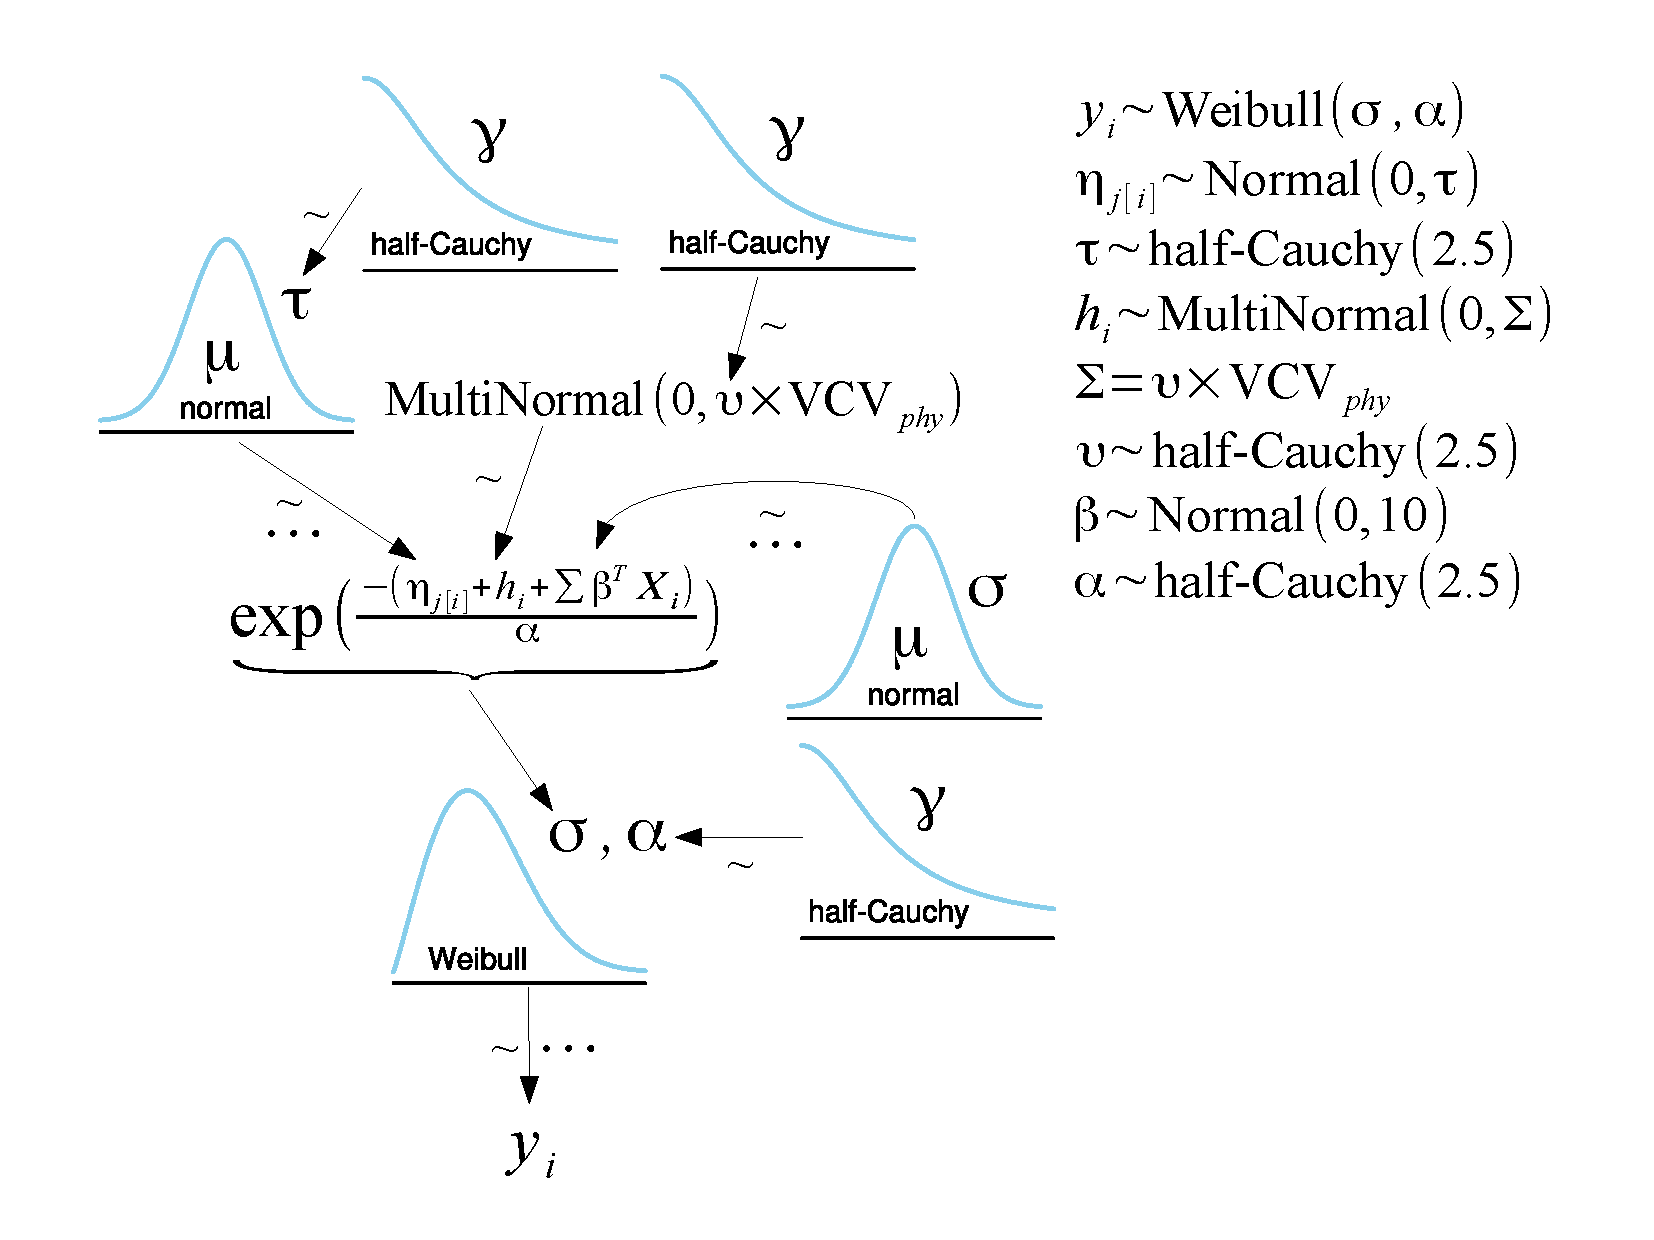
\includegraphics[height = 0.5\textheight, width = \textwidth, keepaspectratio = true]{figure/mammal_survival_model}
  \caption{Graphical depiction of full survival model, save censoring, used here. Exact values for the hyperparameters are presented to the right. The observed duration of the \(i\)th observation is indicated towards the bottom left as \(y_{i}\), which is assumed to follow a Weibull distribution.}
  \label{fig:model_diagram}
\end{figure}


The parameter posteriors were approximated using a Markov-chain Monte Carlo (MCMC) routine implemented in the Stan programming language \citep{2014stan}. Stan implements a Hamiltonian Monte Carlo using a No-U-Turn sampler \citep{Hoffman-Gelman:2011}. Posterior approximation was done using four parallel MCMC chains. Chain convergence was evaluated using the scale reduction factor, \(\hat{R}\). Values of \(\hat{R}\) close to 1, or less than or equal to 1.1, indicate approximate convergence. Convergence means that the chains are approximately stationary and the samples are well mixed \citep{Gelman2013d}.

Both models with and without phylogenetic effects were estimated. Because inverting a large matrix is a memory intense procedure and because the phylogenetic covariance matrix is only assumed known up to a constant, every iteration of the MCMC would involve solving a very large matrix which is not ideal. In order to speed up the MCMC routine, this aspect of the model had to be reparameterized for efficiency purposes. One way of doing this is by using a Cholesky parameterized version of the multivariate normal distribution with a Cholesky decomposed covariance matrix, however because of the size of the covariance matrix this speed up is only minor. Instead, a custom multivariate sampler was used (see Appendix: Code).

For the model without phylogenetic effect the four MCMC chains ran for 2000 steps, with the first 1000 used as warm-up and the last 1000 as samples from the posterior. Because of the added complexity of estimating the phylogenetic effect, all four chains were run 10000 steps thinned to every tenth sample split evenly between warm-up and sampling. 



\subsubsection{Posterior predictive checks}

The most basic assessment of model fit is that simulated data generated using the fitted model should be similar to the observed. This is the idea behind posterior predictive checks. Using the predictors from each of the observed durations, and randomly drawn parameter estimates from their marginal posteriors, a simulated data set \(y^{rep}\) was generated. This process repeated 1000 times and the distribution of \(y^{rep}\) was compared with the observed \(y\) \citep{Gelman2013d}. This was done both graphically and numerically.

An example posterior predictive check used in this study is a graphical comparison of the Kaplan-Meier (K-M) survival curve estimated from the observed data with the survival curves from 1000 simulations. K-M survival curves are non-parametric estimates of the function \(S(t)\) or the probability of a species going extinct given that it has lived to time \(t\) \citep{Kleinbaum2005}. Other posterior predictive checks included comparison of the mean and quantiles of the observed durations to the distributions of the same quantities from the simulations.




\end{document}
